\section{二重积分的换元}

\begin{problem}{计算重积分}{Double-Integrals-Calculation}
    计算下列积分：
    \begin{enumerate}
        \item $\int_{0}^{R} \d x \int_{0}^{\sqrt{R^2-x^2}} \ln(1 + x^2 + y^2) \d y$;
        \item $\int_{0}^{a} \d x \int_{0}^{b} xy(x^2 - y^2) \d y$;
        \item $\int_{0}^{\uppi} \int_{0}^{\uppi} \cos(x + y) \d x \d y$;
        \item $\int_{0}^{\frac{1}{\sqrt{2}}} \d x \int_{x}^{\sqrt{1 - x^2}} xy(x + y) \d y$;
        \item $\int_{0}^{\frac{R}{\sqrt{1+R^2}}} \d x \int_{0}^{Rx} \left(1 + \frac{y^2}{x^2}\right) \d y + \int_{\frac{R}{\sqrt{1+R^2}}}^{R} \d x \int_{0}^{\sqrt{R^2-x^2}} \left(1 + \frac{y^2}{x^2}\right) \d y$.
    \end{enumerate}
\end{problem}

\begin{solution}
    \ansitem{1} 积分区域 $D_1 = \{(x, y) \mid 0 \le x \le R, 0 \le y \le \sqrt{R^2-x^2}\}$ 为第一象限内的 $1/4$ 圆盘。

    \begin{center}
        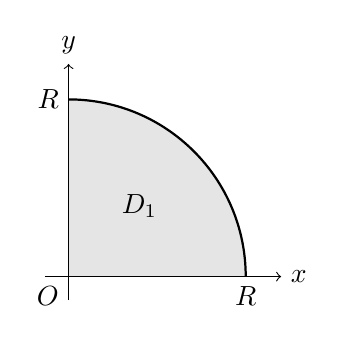
\begin{tikzpicture}[scale=1.5]
            \fill[gray!20] (0,0) -- (1.5,0) arc (0:90:1.5) -- cycle;
            \draw[->] (-0.2,0) -- (1.8,0) node[right] {$x$};
            \draw[->] (0,-0.2) -- (0,1.8) node[above] {$y$};
            \draw[thick] (1.5,0) arc (0:90:1.5);
            \node at (0.6,0.6) {$D_1$};
            \node[below left] at (0,0) {$O$};
            \node[below] at (1.5,0) {$R$};
            \node[left] at (0,1.5) {$R$};
        \end{tikzpicture}
    \end{center}

    采用极坐标变换 $x = r \cos \theta, y = r \sin \theta$，则 $D_1$ 对应 $0 \le \theta \le \frac{\uppi}{2}, 0 \le r \le R$，
    \begin{equation}
        \begin{aligned}
            I_1 & = \int_{0}^{\frac{\uppi}{2}} \d \theta \int_{0}^{R} \ln(1 + r^2) \cdot r \d r \\
                & = \frac{\uppi}{4} \int_{0}^{R} \ln(1 + r^2) \d (1 + r^2)                      \\
                & = \frac{\uppi}{4} \left[ (1 + r^2) \ln(1 + r^2) - (1 + r^2) \right]_0^R.
        \end{aligned}
    \end{equation}
    \begin{equation}
        I_1 = \boxed{\frac{\uppi}{4} \left[ (1 + R^2) \ln(1 + R^2) - R^2 \right]}
    \end{equation}

    \ansitem{2} 积分区域 $D_2 = [0, a] \times [0, b]$ 为矩形区域。

    \begin{center}
        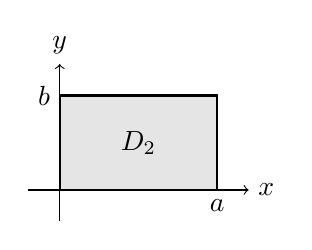
\begin{tikzpicture}[scale=0.8]
            \fill[gray!20] (0,0) rectangle (2.5,1.5);
            \draw[->] (-0.5,0) -- (3,0) node[right] {$x$};
            \draw[->] (0,-0.5) -- (0,2) node[above] {$y$};
            \draw[thick] (0,0) rectangle (2.5,1.5);
            \node at (1.25,0.75) {$D_2$};
            \node[below] at (2.5,0) {$a$};
            \node[left] at (0,1.5) {$b$};
        \end{tikzpicture}
    \end{center}

    直接进行累次积分推导，
    \begin{equation}
        \begin{aligned}
            I_2 & = \int_{0}^{a} x \d x \int_{0}^{b} (x^2 y - y^3) \d y                          \\
                & = \int_{0}^{a} x \left[ \frac{1}{2} x^2 y^2 - \frac{1}{4} y^4 \right]_0^b \d x \\
                & = \int_{0}^{a} \left( \frac{1}{2} b^2 x^3 - \frac{1}{4} b^4 x \right) \d x     \\
                & = \left[ \frac{1}{8} b^2 x^4 - \frac{1}{8} b^4 x^2 \right]_0^a.
        \end{aligned}
    \end{equation}
    \begin{equation}
        I_2 = \boxed{\frac{1}{8} a^2 b^2 (a^2 - b^2)}
    \end{equation}

    \ansitem{3} 积分区域 $D_3 = [0, \uppi] \times [0, \uppi]$ 为正方形区域。

    \begin{center}
        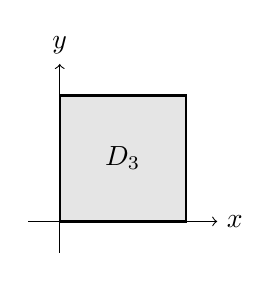
\begin{tikzpicture}[scale=0.8]
            \fill[gray!20] (0,0) rectangle (2,2);
            \draw[->] (-0.5,0) -- (2.5,0) node[right] {$x$};
            \draw[->] (0,-0.5) -- (0,2.5) node[above] {$y$};
            \draw[thick] (0,0) rectangle (2,2);
            \node at (1,1) {$D_3$};
            \node[below] at (2,0) {$\uppi$};
            \node[left] at (0,2) {$\uppi$};
        \end{tikzpicture}
    \end{center}

    计算过程如下，
    \begin{equation}
        \begin{aligned}
            I_3 & = \int_{0}^{\uppi} \d x \int_{0}^{\uppi} \cos(x + y) \d y    \\
                & = \int_{0}^{\uppi} \left[ \sin(x + y) \right]_0^{\uppi} \d x \\
                & = \int_{0}^{\uppi} (\sin(x + \uppi) - \sin x) \d x           \\
                & = \int_{0}^{\uppi} (-2 \sin x) \d x = [2 \cos x]_0^{\uppi}.
        \end{aligned}
    \end{equation}
    \begin{equation}
        I_3 = \boxed{-4}
    \end{equation}

    \ansitem{4} 积分区域 $D_4 = \{(x, y) \mid 0 \le x \le \frac{1}{\sqrt{2}}, x \le y \le \sqrt{1-x^2}\}$ 为单位圆在第一象限内由射线 $y=x$ 与 $y$ 轴围成的扇形。

    \begin{center}
        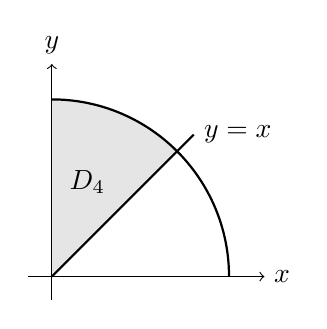
\begin{tikzpicture}[scale=1.5]
            \fill[gray!20] (0,0) -- (45:1.5) arc (45:90:1.5) -- cycle;
            \draw[->] (-0.2,0) -- (1.8,0) node[right] {$x$};
            \draw[->] (0,-0.2) -- (0,1.8) node[above] {$y$};
            \draw[thick] (1.5,0) arc (0:90:1.5);
            \draw[thick] (0,0) -- (45:1.7) node[right] {$y=x$};
            \node at (0.3,0.8) {$D_4$};
        \end{tikzpicture}
    \end{center}

    利用极坐标，区域对应 $\frac{\uppi}{4} \le \theta \le \frac{\uppi}{2}, 0 \le r \le 1$，
    \begin{equation}
        \begin{aligned}
            I_4 & = \int_{\frac{\uppi}{4}}^{\frac{\uppi}{2}} \d \theta \int_{0}^{1} (r^2 \cos \theta \sin \theta) (r \cos \theta + r \sin \theta) \cdot r \d r      \\
                & = \left( \int_{0}^{1} r^4 \d r \right) \int_{\frac{\uppi}{4}}^{\frac{\uppi}{2}} (\sin \theta \cos^2 \theta + \sin^2 \theta \cos \theta) \d \theta \\
                & = \frac{1}{5} \left[ -\frac{1}{3} \cos^3 \theta + \frac{1}{3} \sin^3 \theta \right]_{\frac{\uppi}{4}}^{\frac{\uppi}{2}}                           \\
                & = \frac{1}{15} \left[ (0 + 1) - \left( -\frac{\sqrt{2}}{4} + \frac{\sqrt{2}}{4} \right) \right].
        \end{aligned}
    \end{equation}
    \begin{equation}
        I_4 = \boxed{\frac{1}{15}}
    \end{equation}

    \ansitem{5} 该积分表示在由 $y=Rx$ 与 $x^2+y^2=R^2$ 围成的第一象限扇形区域 $D_5$ 上的积分。设 $\alpha = \arctan R$。

    \begin{center}
        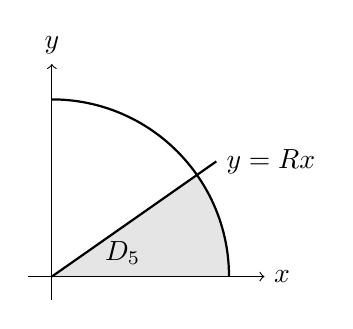
\begin{tikzpicture}[scale=1.5]
            \fill[gray!20] (0,0) -- (1.5,0) arc (0:35:1.5) -- cycle;
            \draw[->] (-0.2,0) -- (1.8,0) node[right] {$x$};
            \draw[->] (0,-0.2) -- (0,1.8) node[above] {$y$};
            \draw[thick] (1.5,0) arc (0:90:1.5);
            \draw[thick] (0,0) -- (35:1.7) node[right] {$y=Rx$};
            \node at (0.6,0.2) {$D_5$};
        \end{tikzpicture}
    \end{center}

    极坐标下 $\frac{y}{x} = \tan \theta$，区域为 $0 \le \theta \le \alpha, 0 \le r \le R$，
    \begin{equation}
        \begin{aligned}
            I_5 & = \int_{0}^{\alpha} \d \theta \int_{0}^{R} (1 + \tan^2 \theta) r \d r          \\
                & = \left( \int_{0}^{R} r \d r \right) \int_{0}^{\alpha} \sec^2 \theta \d \theta \\
                & = \frac{1}{2} R^2 \cdot [ \tan \theta ]_0^{\alpha}                             \\
                & = \frac{1}{2} R^2 \cdot R.
        \end{aligned}
    \end{equation}
    \begin{equation}
        I_5 = \boxed{\frac{1}{2} R^3}
    \end{equation}
\end{solution}


\begin{problem}{二重积分的计算}{Double-Integral-Calculation}
    计算下列二重积分：
    \begin{enumerate}
        \item $\iint_{D} \sqrt{x^{2}+y^{2}} \d x \d y$，其中 $D: x^{2}+y^{2} \leqslant x+y$；
        \item $\iint_{D} \sqrt{\frac{x^{2}}{a^{2}}+\frac{y^{2}}{b^{2}}} \d x \d y$，其中 $D: \frac{x^{2}}{a^{2}}+\frac{y^{2}}{b^{2}}=4, y=0, y=x$ 所围成的第一象限部分；
        \item $\iint_{D} (x^{2}+y^{2}) \d x \d y$，其中 $D$ 为由 $xy=1, xy=2, y=x, y=2x$ 围成的第一象限部分；
        \item $\iint_{D} \d x \d y$，其中 $D$ 为由 $y^{2}=ax, y^{2}=bx, x^{2}=my, x^{2}=ny$ 围成的区域 ($a>b>0, m>n>0$)；
        \item $\iint_{D} xy \d x \d y$，其中 $D$ 为 $xy=a, xy=b, y^{2}=cx, y^{2}=dx$ 围成的第一象限部分 ($0<a<b, 0<c<d$)；
        \item $\iint_{D} 4xy \d x \d y$，其中 $D: x^{4}+y^{4} \leqslant 1, x \geqslant 0, y \geqslant 0$ 围成的区域；
        \item $\iint_{D} \frac{x^{2}-y^{2}}{\sqrt{x+y+3}} \d x \d y$，其中 $D: |x|+|y| \leqslant 1$；
        \item $\iint_{D} \sin \frac{y}{x+y} \d x \d y$，其中 $D$ 为由直线 $x+y=1, x=0, y=0$ 围成的区域；
        \item $\iint_{D} |xy| \d x \d y$，其中 $D = \{(x,y) : x^2 + y^2 \leqslant a^2\}$。
    \end{enumerate}
\end{problem}

\begin{solution}
    \ansitem{1}

    利用极坐标变换 $x = r \cos \theta$、$y = r \sin \theta$，区域 $D$ 的边界方程为 $r^2 \leqslant r(\cos \theta + \sin \theta)$，即 $r \leqslant \sqrt{2} \cos(\theta - \uppi/4)$，对应的辐角范围为 $\theta \in [-\uppi/4, 3\uppi/4]$。积分计算如下：
    \begin{equation}
        \begin{aligned}
            \iint_D \sqrt{x^2+y^2} \d x \d y & = \int_{-\uppi/4}^{3\uppi/4} \d \theta \int_0^{\sqrt{2}\cos(\theta - \uppi/4)} r^2 \d r             \\
                                             & = \frac{1}{3} \int_{-\uppi/2}^{\uppi/2} (\sqrt{2}\cos \phi)^3 \d \phi \label{eq:int-1-step}         \\
                                             & = \frac{4\sqrt{2}}{3} \int_0^{\uppi/2} \cos^3 \phi \d \phi = \frac{4\sqrt{2}}{3} \cdot \frac{2}{3}.
        \end{aligned}
    \end{equation}
    \begin{equation}
        \iint_D \sqrt{x^2+y^2} \d x \d y = \boxed{\frac{8\sqrt{2}}{9}}
    \end{equation}

    \ansitem{2}

    引入广义极坐标变换 $x = ar\cos\theta$、$y = br\sin\theta$，对应的雅可比行列式绝对值为 $abr$。区域 $D$ 在新平面中对应 $r \in [0, 2]$ 且 $\theta \in [0, \arctan(a/b)]$。计算积分：
    \begin{equation}
        \begin{aligned}
            \iint_D \sqrt{\frac{x^2}{a^2} + \frac{y^2}{b^2}} \d x \d y & = \int_0^{\arctan(a/b)} \d \theta \int_0^2 r \cdot abr \d r      \\
                                                                       & = ab \arctan\frac{a}{b} \cdot \left[ \frac{1}{3}r^3 \right]_0^2.
        \end{aligned}
    \end{equation}
    \begin{equation}
        \iint_D \sqrt{\frac{x^2}{a^2} + \frac{y^2}{b^2}} \d x \d y = \boxed{\frac{8}{3}ab \arctan\frac{a}{b}}
    \end{equation}

    \ansitem{3}

    作变量替换 $u = xy$、$v = y/x$，则 $x^2+y^2 = u/v + uv$，雅可比行列式绝对值为 $\frac{1}{2v}$。变换后区域为 $[1, 2] \times [1, 2]$：
    \begin{equation}
        \begin{aligned}
            \iint_D (x^2+y^2) \d x \d y & = \int_1^2 \d u \int_1^2 \left( \frac{u}{v} + uv \right) \frac{1}{2v} \d v                                \\
                                        & = \frac{1}{2} \int_1^2 u \d u \int_1^2 \left( \frac{1}{v^2} + 1 \right) \d v \label{eq:int-3-step}        \\
                                        & = \frac{1}{2} \cdot \frac{3}{2} \cdot \left[ v - \frac{1}{v} \right]_1^2 = \frac{3}{4} \cdot \frac{3}{2}.
        \end{aligned}
    \end{equation}
    \begin{equation}
        \iint_D (x^2+y^2) \d x \d y = \boxed{\frac{9}{8}}
    \end{equation}

    \ansitem{4}

    作代换 $u = y^2/x$、$v = x^2/y$，此时 $u \in [b, a]$，$v \in [n, m]$。变换的雅可比行列式满足
    \begin{equation}
        \frac{\partial(u,v)}{\partial(x,y)} = \begin{vmatrix} -y^2/x^2 & 2y/x \\ 2x/y & -x^2/y^2 \end{vmatrix} = 1 - 4 = -3.
    \end{equation}
    故 $\d x \d y = \frac{1}{3} \d u \d v$，积分为
    \begin{equation}
        \iint_D \d x \d y = \frac{1}{3} \int_b^a \d u \int_n^m \d v = \frac{1}{3}(a-b)(m-n).
    \end{equation}
    \begin{equation}
        \iint_D \d x \d y = \boxed{\frac{1}{3}(a-b)(m-n)}
    \end{equation}

    \ansitem{5}

    作代换 $u = xy$、$v = y^2/x$，其中 $u \in [a, b]$、$v \in [c, d]$。其雅可比行列式满足
    \begin{equation}
        \frac{\partial(u,v)}{\partial(x,y)} = \begin{vmatrix} y & x \\ -y^2/x^2 & 2y/x \end{vmatrix} = \frac{3y^2}{x} = 3v.
    \end{equation}
    则 $\d x \d y = \frac{1}{3v} \d u \d v$，积分为
    \begin{equation}
        \begin{aligned}
            \iint_D xy \d x \d y & = \int_a^b \d u \int_c^d u \cdot \frac{1}{3v} \d v                       \\
                                 & = \frac{1}{3} \cdot \left[ \frac{1}{2}u^2 \right]_a^b \cdot [\ln v]_c^d.
        \end{aligned}
    \end{equation}
    \begin{equation}
        \iint_D xy \d x \d y = \boxed{\frac{1}{6}(b^2-a^2) \ln \frac{d}{c}}
    \end{equation}

    \ansitem{6}

    采用广义极坐标变换 $x^2 = r \cos \theta$、$y^2 = r \sin \theta$，变换的雅可比行列式绝对值满足 $4xy \d x \d y = r \d r \d \theta$。区域 $D$ 对应 $r \in [0, 1]$ 且 $\theta \in [0, \uppi/2]$。积分为
    \begin{equation}
        \iint_D 4xy \d x \d y = \int_0^{\uppi/2} \d \theta \int_0^1 r \d r = \frac{\uppi}{2} \cdot \frac{1}{2}.
    \end{equation}
    \begin{equation}
        \iint_D 4xy \d x \d y = \boxed{\frac{\uppi}{4}}
    \end{equation}

    \ansitem{7}

    积分区域 $D: |x|+|y| \leqslant 1$ 关于直线 $y=x$ 对称。将被积函数中的 $x$ 与 $y$ 对换，根据对称性有
    \begin{equation}
        I = \iint_D \frac{x^2-y^2}{\sqrt{x+y+3}} \d x \d y = \iint_D \frac{y^2-x^2}{\sqrt{y+x+3}} \d y \d x = -I,
    \end{equation}
    由此可推得 $I = 0$。最终结果为
    \begin{equation}
        \iint_D \frac{x^2-y^2}{\sqrt{x+y+3}} \d x \d y = \boxed{0}
    \end{equation}

    \ansitem{8}

    引入变换 $u = x+y$、$v = y$，则 $\d x \d y = \d u \d v$。区域 $D$ 映射为 $0 \leqslant u \leqslant 1$，$0 \leqslant v \leqslant u$。积分如下：
    \begin{equation}
        \begin{aligned}
            \iint_D \sin \frac{y}{x+y} \d x \d y & = \int_0^1 \d u \int_0^u \sin \frac{v}{u} \d v                                                 \\
                                                 & = \int_0^1 \left[ -u \cos \frac{v}{u} \right]_{v=0}^{v=u} \d u = (1 - \cos 1) \int_0^1 u \d u.
        \end{aligned}
    \end{equation}
    \begin{equation}
        \iint_D \sin \frac{y}{x+y} \d x \d y = \boxed{\frac{1}{2}(1 - \cos 1)}
    \end{equation}

    \ansitem{9}

    由于积分区域 $D$ 及被积函数 $|xy|$ 在四个象限内完全对称，可仅计算第一象限部分 $D_1$ 并乘以 $4$：
    \begin{equation}
        \begin{aligned}
            \iint_D |xy| \d x \d y & = 4 \iint_{D_1} xy \d x \d y                                                                   \\
                                   & = 4 \int_0^{\uppi/2} \sin \theta \cos \theta \d \theta \int_0^a r^3 \d r \label{eq:int-9-step} \\
                                   & = 4 \cdot \frac{1}{2} \cdot \frac{a^4}{4}.
        \end{aligned}
    \end{equation}
    \begin{equation}
        \iint_D |xy| \d x \d y = \boxed{\frac{a^4}{2}}
    \end{equation}
\end{solution}


\begin{problem}{平面图形面积}{Plane-Area-Calculation}
    求下列曲线所围成的平面区域的面积：
    \begin{enumerate}
        \item $x^2 + 2y^2 = 3$ 和 $xy = 1$（不含原点部分）；
        \item $(x - y)^2 + x^2 = a^2$ ($a > 0$)；
        \item 由直线 $x + y = a, x + y = b, y = kx$ 和 $y = m x$ ($0 < a < b, 0 < k < m$) 围成的平面区域。
    \end{enumerate}
\end{problem}

\begin{solution}
    \ansitem{1} 联立方程组可得交点为 $(1, 1)$、$(\sqrt{2}, 1/\sqrt{2})$、$(-1, -1)$ 及 $(-\sqrt{2}, -1/\sqrt{2})$。

    由于图形关于原点对称，总面积 $S$ 为第一象限部分面积 $S_1$ 的两倍。在区间 $[1, \sqrt{2}]$ 上，椭圆弧位于双曲线弧上方，则有
    \begin{equation}
        S_1 = \int_{1}^{\sqrt{2}} \left( \sqrt{\frac{3 - x^2}{2}} - \frac{1}{x} \right) \d x = \frac{1}{\sqrt{2}} \int_{1}^{\sqrt{2}} \sqrt{3 - x^2} \d x - \ln \sqrt{2}.
    \end{equation}
    计算其中的定积分：
    \begin{equation}
        \begin{aligned}
            \int_{1}^{\sqrt{2}} \sqrt{3 - x^2} \d x & = \left[ \frac{x}{2} \sqrt{3 - x^2} + \frac{3}{2} \arcsin \frac{x}{\sqrt{3}} \right]_{1}^{\sqrt{2}}                                                       \\
                                                    & = \left( \frac{\sqrt{2}}{2} + \frac{3}{2} \arcsin \sqrt{\frac{2}{3}} \right) - \left( \frac{\sqrt{2}}{2} + \frac{3}{2} \arcsin \frac{1}{\sqrt{3}} \right) \\
                                                    & = \frac{3}{2} \left( \arcsin \sqrt{\frac{2}{3}} - \arcsin \frac{1}{\sqrt{3}} \right).
        \end{aligned}
    \end{equation}
    利用三角恒等式 $\arcsin \sqrt{2/3} - \arcsin 1/\sqrt{3} = \arcsin 1/3$，得 $S = 2 \left( \frac{3}{2\sqrt{2}} \arcsin \frac{1}{3} - \frac{1}{2} \ln 2 \right)$。
    \begin{equation}
        S = \boxed{\frac{3\sqrt{2}}{2} \arcsin \frac{1}{3} - \ln 2}
    \end{equation}

    \ansitem{2} 令 $u = x$、$v = y - x$，该坐标变换的雅可比行列式绝对值为 $|J| = 1$。

    在此变换下，原方程化为 $u^2 + v^2 = a^2$。故平面区域的面积为
    \begin{equation}
        S = \iint_{u^2 + v^2 \le a^2} 1 \cdot \d u \d v = \uppi a^2.
    \end{equation}
    \begin{equation}
        S = \boxed{\uppi a^2}
    \end{equation}

    \ansitem{3} 令 $u = x + y$、$v = y/x$。由此解得 $x = \frac{u}{1+v}$，$y = \frac{uv}{1+v}$。

    计算该变换的雅可比行列式：
    \begin{equation}
        J = \frac{\partial(x, y)}{\partial(u, v)} = \det \begin{pmatrix} \frac{1}{1+v} & -\frac{u}{(1+v)^2} \\ \frac{v}{1+v} & \frac{u}{(1+v)^2} \end{pmatrix} = \frac{u}{(1+v)^2}.
    \end{equation}
    区域 $D$ 在 $uv$ 平面上对应于矩形区域 $[a, b] \times [k, m]$。面积为
    \begin{equation}
        \begin{aligned}
            S & = \int_{k}^{m} \int_{a}^{b} \frac{u}{(1+v)^2} \d u \d v = \left( \int_{a}^{b} u \d u \right) \left( \int_{k}^{m} \frac{1}{(1+v)^2} \d v \right) \\
              & = \frac{b^2 - a^2}{2} \left[ -\frac{1}{1+v} \right]_{k}^{m} = \frac{b^2 - a^2}{2} \left( \frac{1}{1+k} - \frac{1}{1+m} \right).
        \end{aligned}
    \end{equation}
    \begin{equation}
        S = \boxed{\frac{(b^2 - a^2)(m - k)}{2(1+k)(1+m)}}
    \end{equation}
\end{solution}

\begin{note}{}{}
    刚才用到的三角恒等式 $\arcsin \sqrt{2/3} - \arcsin 1/\sqrt{3} = \arcsin 1/3$ 可以通过以下方法验证：
    设 $\alpha = \arcsin \sqrt{2/3}$，$\beta = \arcsin 1/\sqrt{3}$，则 $\sin \alpha = \sqrt{2/3}$，$\sin \beta = 1/\sqrt{3}$。
    根据正弦差角公式 $\sin(\alpha - \beta) = \sin \alpha \cos \beta - \cos \alpha \sin \beta$，我们可以计算 $\sin(\alpha - \beta)$：
    \begin{equation}
        \begin{aligned}
            \sin(\alpha - \beta) & = \sqrt{\frac{2}{3}} \cdot \sqrt{1 - \left(\frac{1}{\sqrt{3}}\right)^2} - \sqrt{1 - \left(\sqrt{\frac{2}{3}}\right)^2} \cdot \frac{1}{\sqrt{3}} \\
                                 & = \sqrt{\frac{2}{3}} \cdot \sqrt{\frac{2}{3}} - \sqrt{\frac{1}{3}} \cdot \frac{1}{\sqrt{3}} = \frac{2}{3} - \frac{1}{3} = \frac{1}{3}.
        \end{aligned}
    \end{equation}
    因此，$\sin(\alpha - \beta) = 1/3$，这验证了 $\alpha - \beta = \arcsin 1/3$，即 $\arcsin \sqrt{2/3} - \arcsin 1/\sqrt{3} = \arcsin 1/3$。
\end{note}

\begin{problem}{二重积分的不等式}{Double-Integral-Comparison}
    证明：
    \begin{equation}
        \iint_{x^2+y^2 \le 1} \e^{x^2+y^2} \d x \d y \le \left[ \int_{-\frac{\sqrt{\uppi}}{2}}^{\frac{\sqrt{\uppi}}{2}} \e^{x^2} \d x \right]^2.
    \end{equation}
\end{problem}

\begin{myproof}

    设区域 $D_1 = \{ (x, y) \mid x^2 + y^2 \le 1 \}$，其面积为 $S(D_1) = \uppi$。

    设区域 $D_2 =  \left\{ (x, y)  \mid  -\frac{\sqrt{\uppi}}{2}  \le  x  \le  \frac{\sqrt{\uppi}}{2},  -\frac{\sqrt{\uppi}}{2}  \le  y  \le  \frac{\sqrt{\uppi}}{2}  \right\}$，其面积为 $S(D_2) = (\sqrt{\uppi})^2 = \uppi$。
    利用累次积分性质可知
    \begin{equation}
        \left[ \int_{-\frac{\sqrt{\uppi}}{2}}^{\frac{\sqrt{\uppi}}{2}} \e^{x^2} \d x \right]^2 = \int_{-\frac{\sqrt{\uppi}}{2}}^{\frac{\sqrt{\uppi}}{2}} \e^{x^2} \d x \int_{-\frac{\sqrt{\uppi}}{2}}^{\frac{\sqrt{\uppi}}{2}} \e^{y^2} \d y = \iint_{D_2} \e^{x^2+y^2} \d x \d y.
    \end{equation}
    考察两积分之差
    \begin{equation}
        \label{eq:diff-integral-01}
        \iint_{D_2} \e^{x^2+y^2} \d \sigma - \iint_{D_1} \e^{x^2+y^2} \d \sigma = \iint_{D_2 \setminus D_1} \e^{x^2+y^2} \d \sigma - \iint_{D_1 \setminus D_2} \e^{x^2+y^2} \d \sigma.
    \end{equation}
    由于 $S(D_1) = S(D_2)$，故 $S(D_2 \setminus D_1) = S(D_1 \setminus D_2)$。
    在区域 $D_1 \setminus D_2$ 中，$x^2 + y^2 \le 1$，故被积函数满足 $\e^{x^2+y^2} \le \e$；
    在区域 $D_2 \setminus D_1$ 中，$x^2 + y^2 > 1$，故被积函数满足 $\e^{x^2+y^2} > \e$。
    结合面积相等的条件，由积分估值定理可得
    \begin{equation}
        \iint_{D_2 \setminus D_1} \e^{x^2+y^2} \d \sigma > \e \cdot S(D_2 \setminus D_1) = \e \cdot S(D_1 \setminus D_2) \ge \iint_{D_1 \setminus D_2} \e^{x^2+y^2} \d \sigma.
    \end{equation}
    由 \zcref{eq:diff-integral-01} 可知 $\iint_{D_2} \e^{x^2+y^2} \d \sigma > \iint_{D_1} \e^{x^2+y^2} \d \sigma$，即
    \begin{equation}
        \boxed{\iint_{x^2+y^2 \le 1} \e^{x^2+y^2} \d x \d y \le \left[ \int_{-\frac{\sqrt{\uppi}}{2}}^{\frac{\sqrt{\uppi}}{2}} \e^{x^2} \d x \right]^2}
    \end{equation}
\end{myproof}

\begin{note}{}{}
    上述解析中的 $D_1 \setminus D_2$ 指的是集合 $D_1$ 中不包含在 $D_2$ 中的部分，即 $D_1$ 与 $D_2$ 的差集。
    此外还有 $D_1 - D_2$ 的写法，这两个表达式在集合论中是等价的。

\end{note}


\begin{problem}{Cauchy-Schwarz 不等式应用}{Cauchy-Schwarz-Application}
    设 $f(x)$ 在 $[0, 1]$ 上连续，证明：
    \begin{equation}
        \int_0^1 \e^{f(x)} \d x \cdot \int_0^1 \e^{-f(y)} \d y \ge 1.
    \end{equation}
\end{problem}

\begin{myproof}
    令 $g(x) = \e^{\frac{1}{2} f(x)}$，$h(x) = \e^{-\frac{1}{2} f(x)}$。
    由 Cauchy-Schwarz 不等式可知
    \begin{equation}
        \left( \int_0^1 g^2(x) \d x \right) \left( \int_0^1 h^2(x) \d x \right) \ge \left( \int_0^1 g(x) h(x) \d x \right)^2.
    \end{equation}
    将函数定义代入上式
    \begin{equation}
        \int_0^1 \e^{f(x)} \d x \cdot \int_0^1 \e^{-f(x)} \d x \ge \left( \int_0^1 \e^{\frac{1}{2} f(x)} \cdot \e^{-\frac{1}{2} f(x)} \d x \right)^2 = \left( \int_0^1 1 \d x \right)^2 = 1.
    \end{equation}
    由于定积分的结果与积分变量的符号无关，即 $\int_0^1 \e^{-f(x)} \d x = \int_0^1 \e^{-f(y)} \d y$，故有
    \begin{equation}
        \boxed{\int_0^1 \e^{f(x)} \d x \cdot \int_0^1 \e^{-f(y)} \d y \ge 1}
    \end{equation}
\end{myproof}

\begin{note}{Cauchy-Schwarz 不等式}{Cauchy-Schwarz Inequality}
    上述解题过程中使用的 Cauchy-Schwarz 不等式是指对于任意实数函数 $g(x)$ 和 $h(x)$，在区间 $[a, b]$ 上满足
    \begin{equation}
        \left( \int_a^b g^2(x) \d x \right) \left( \int_a^b h^2(x) \d x \right) \ge \left( \int_a^b g(x) h(x) \d x \right)^2.
    \end{equation}

    想证明这个不等式，可以考虑定义一个函数 $F(t) = \int_a^b (g(x) - t h(x))^2 \d x$，由于 $F(t) \ge 0$ 对任意实数 $t$ 都成立，展开 $F(t)$ 可得
    \begin{equation}
        F(t) = \int_a^b g^2(x) \d x - 2t \int_a^b g(x) h(x) \d x + t^2 \int_a^b h^2(x) \d x.
    \end{equation}
    由于 $F(t)$ 是一个关于 $t$ 的二次函数，并且 $F(t) \ge 0$，其判别式必须小于或等于零，即
    \begin{equation}
        \Delta = \left( -2 \int_a^b g(x) h(x) \d x \right)^2 - 4 \left( \int_a^b g^2(x) \d x \right) \left( \int_a^b h^2(x) \d x \right) \le 0,
    \end{equation}
    从而得出 Cauchy-Schwarz 不等式。

\end{note}


\begin{problem}{奇函数重积分不等式}{Odd-Function-Inequality}
    设 $f(x)$ 为连续的奇函数，证明：
    \begin{equation}
        \iint_{|x|+|y| \le 1} \e^{f(x+y)} \d x \d y \ge 2.
    \end{equation}
\end{problem}

\begin{myproof}
    设积分区域 $D = \{ (x, y) \mid |x| + |y| \le 1 \}$。引入变量代换
    \begin{equation}
        \begin{cases} u = x + y \\ v = x - y \end{cases} \implies \begin{cases} x = \frac{1}{2}(u + v) \\ y = \frac{1}{2}(u - v) \end{cases},
    \end{equation}
    计算雅可比行列式的绝对值为 $|J| = \left| \frac{\partial(x, y)}{\partial(u, v)} \right| = \frac{1}{2}$。
    变换后的积分区域为 $D' = \{ (u, v) \mid |u| \le 1, |v| \le 1 \}$，则
    \begin{equation}
        \iint_D \e^{f(x+y)} \d x \d y = \int_{-1}^1 \int_{-1}^1 \e^{f(u)} \cdot \frac{1}{2} \d v \d u = \int_{-1}^1 \e^{f(u)} \d u.
    \end{equation}
    利用 $f(x)$ 为奇函数（即 $f(-u) = -f(u)$）的性质，对积分进行拆分
    \begin{equation}
        \int_{-1}^1 \e^{f(u)} \d u = \int_{-1}^0 \e^{f(u)} \d u + \int_0^1 \e^{f(u)} \d u = \int_0^1 \left( \e^{f(u)} + \e^{-f(u)} \right) \d u.
    \end{equation}
    由算术—几何平均值不等式可知 $\e^{f(u)} + \e^{-f(u)} \ge 2\sqrt{\e^{f(u)} \cdot \e^{-f(u)}} = 2$，代入积分式
    \begin{equation}
        \int_0^1 \left( \e^{f(u)} + \e^{-f(u)} \right) \d u \ge \int_0^1 2 \d u = 2.
    \end{equation}
    由此证得
    \begin{equation}
        \boxed{\iint_{|x|+|y| \le 1} \e^{f(x+y)} \d x \d y \ge 2}
    \end{equation}
\end{myproof}


\begin{problem}{二重积分与变量代换}{Double-Integral-Substitution}
    设 $f(t)$ 为连续函数，求证：
    \begin{equation}
        \iint_D f(x - y) \d x \d y = \int_{-A}^A f(t)(A - |t|) \d t
    \end{equation}
    其中 $D$：$|x| \le \frac{A}{2}$、$|y| \le \frac{A}{2}$，$A > 0$ 为常数。
\end{problem}

\begin{myproof}
    根据题意，积分区域 $D$ 是一个正方形。将二重积分转化为累次积分
    \begin{equation}
        \label{eq:step-1}
        \iint_D f(x - y) \d x \d y = \int_{-\frac{A}{2}}^{\frac{A}{2}} \d x \int_{-\frac{A}{2}}^{\frac{A}{2}} f(x - y) \d y.
    \end{equation}
    对于内层关于 $y$ 的积分，令 $t = x - y$，则有 $\d y = -\d t$。当 $y = -\frac{A}{2}$ 时，$t = x + \frac{A}{2}$；当 $y = \frac{A}{2}$ 时，$t = x - \frac{A}{2}$。代入 \zcref{eq:step-1} 可得
    \begin{equation}
        \label{eq:step-2}
        \iint_D f(x - y) \d x \d y = \int_{-\frac{A}{2}}^{\frac{A}{2}} \d x \int_{x - \frac{A}{2}}^{x + \frac{A}{2}} f(t) \d t.
    \end{equation}
    在 $(x, t)$ 平面上，积分区域由 $-\frac{A}{2} \le x \le \frac{A}{2}$ 与 $x - \frac{A}{2} \le t \le x + \frac{A}{2}$ 围成。交换 \zcref{eq:step-2} 中的积分次序，需根据 $t$ 的取值范围进行分段推导
    \begin{equation}
        \begin{aligned}
            \iint_D f(x - y) \d x \d y & = \int_{-A}^{0} f(t) \d t \int_{-\frac{A}{2}}^{t + \frac{A}{2}} \d x + \int_{0}^{A} f(t) \d t \int_{t - \frac{A}{2}}^{\frac{A}{2}} \d x                                                    \\
                                       & = \int_{-A}^{0} f(t) \left[ \left( t + \frac{A}{2} \right) - \left( -\frac{A}{2} \right) \right] \d t + \int_{0}^{A} f(t) \left[ \frac{A}{2} - \left( t - \frac{A}{2} \right) \right] \d t \\
                                       & = \int_{-A}^{0} f(t) (A + t) \d t + \int_{0}^{A} f(t) (A - t) \d t.
        \end{aligned}
    \end{equation}
    注意到当 $t \in [-A, 0]$ 时，$A + t = A - |t|$；当 $t \in [0, A]$ 时，$A - t = A - |t|$。因此
    \begin{equation}
        \iint_D f(x - y) \d x \d y = \int_{-A}^0 f(t) (A - |t|) \d t + \int_0^A f(t) (A - |t|) \d t.
    \end{equation}
    整理即得欲证结论
    \begin{equation}
        \iint_D f(x - y) \d x \d y = \boxed{\int_{-A}^A f(t) (A - |t|) \d t}
    \end{equation}
\end{myproof}
